\begin{figure}[p]
\centering
\begin{tikzpicture}[
box/.style={draw,rounded corners,align=center,text width=12.7cm,
 inner sep=8pt},arrow/.style={->,thick}]
\node[box,fill=blue!5] (boundary) at (0,0)
{Original balanced boundary character (BCE1--4)\\
\(U_{\alpha}=3^m,\quad\alpha=(3,(1)_p),\quad1\le m<r\).\\
This is an idele action; the collision operator is separately
\(F_M(T)=9cz,\ F_M^2=0\).};
\node[box,fill=blue!5] (extension) at (0,-2.5)
{Original cotangent extension (BCE6)\\
\(0\longrightarrow M\xrightarrow{d_M}\Omega
\xrightarrow{\rho}O/9\longrightarrow0,\qquad9q=3d_M(z)\).};
\draw[arrow] (boundary) -- node[right,font=\small]
{compare through \(3^mI-F\)} (extension);
\node[box,fill=green!5] (torsion) at (0,-5)
{Exact connecting map (BCE15--16)\\
\(m=1:\ \delta_1=0.\qquad
m\ge2:\ \delta_m(1)=[3^{m-1}z]\), of order \(3\).\\
The first nonzero mixed count is \(m=2\), at tensor order \(r=3\).};
\draw[arrow] (extension) -- (torsion);
\node[draw,rounded corners,align=center,text width=5.7cm,
inner sep=8pt,fill=green!5] (detect) at (-3.55,-8)
{Torsion receiver (BCE19--20)\\[3pt]
\(\displaystyle\lambda_m([x])
=\frac{x_z}{3^m}+\frac{9c\,x_T}{3^{2m}}\pmod O\)\\[5pt]
\(\lambda_m\delta_m(1)=1/3\pmod O\ne0.\)};
\node[draw,rounded corners,align=center,text width=5.7cm,
inner sep=8pt,fill=orange!8] (kill) at (3.55,-8)
{Cotangent receiver (BCE22--25)\\[3pt]
\(\kappa_m^1=\kappa+3^{-m}\kappa F_M\)\\
exists exactly when \(27c\in3^mO\).\\[5pt]
Where defined, \((\kappa_m^1)_*\delta_m=0\).};
\draw[arrow] (torsion.south) -- ++(0,-.35) -| (detect.north);
\draw[arrow] (torsion.south) -- ++(0,-.35) -| (kill.north);
\node[box,fill=gray!5] at (0,-10.8)
{Every map retains its support labels (BCE28). A killed top-supported
class returns to \(e=(0,1_L)\), while \(\tau=(0,0_L)\) remains distinct.\\
The torsion pairing takes values in \(\mathbb Q_3/\mathbb Z_3\);
it asserts no positivity of the original Weil form.};
\end{tikzpicture}
\caption{The two computed receivers of the mixed collision class,
with original constants and signs. The top box uses the Connes--Consani--Marcolli
adelic conventions through the published GSB proof; the coefficient
extension is the original CFF construction. The figure depicts
operator comparisons, not an identification of idele dilation with
prismatic Frobenius. All proofs and exact source maps are BCE1--28.}
\end{figure}

\begin{figure}[p]
\centering
\begin{tikzpicture}[
box/.style={draw,rounded corners,align=center,text width=12.7cm,
 inner sep=8pt},arrow/.style={->,thick}]
\node[box,fill=blue!5] (original) at (0,0)
{Original prism and twist (BCE29--33)\\
\(d=3+\epsilon,\quad d^m=3^m+m3^{m-1}\epsilon,\quad
\phi(e_*)=e_*/d.\)\\
The term \(m3^{m-1}\epsilon\) remains in every division.};
\node[box,fill=blue!5] (domain) at (0,-2.8)
{Exact local domain and differential (BCE32--34)\\
\(N_mC=3^{m+\eta_m}O\,1\oplus O\epsilon
\oplus3^{h_m}OT\oplus Oz,\qquad J_m=[N_mC
\xrightarrow{\ \phi/d^m-\iota\ }C].\)\\
\(\eta_m=1\) for \(3\nmid m\), and \(0\) otherwise;
\(h_m=\max(0,m-2-v_3(c))\), with \(h_m=0\) for \(c=0\).};
\draw[arrow] (original) -- (domain);
\node[box,fill=orange!8] (old) at (0,-5.7)
{The earlier connecting class has an explicit primitive (BCE38--40)\\
\(\delta_m(1)=[3^{m-1}z]\longmapsto[-3^{m-1}z]=0,\quad m\ge2,\)\\
\((\phi/d^m-\iota)(3^{m-1}z)=-3^{m-1}z.\)};
\draw[arrow] (domain) -- (old);
\node[box,fill=green!5] (survive) at (0,-8.4)
{The complete surviving local groups (BCE35--37)\\
\(H^0J_m(C)=0,\qquad
H^1J_m(C)=(O/3^{\eta_m})[1]\oplus(O/3^{h_m})[T].\)\\
The constant class measures the exact filtered quotient defect\\
\(N_mO/q(N_mC)=3^mO/3^{m+\eta_m}O.\)};
\draw[arrow] (domain.east) -- ++(.5,0) |- (survive.east);
\node[box,fill=gray!5] at (0,-11.4)
{Completion with the transported filtration preserves these
groups, with an explicit return (BCE42--45).
Recomputing the preimage filtration on the
quotient loses exactly the defect \(Q_m\cong H^1J_m(C)\).\\
These are local prism calculations. Absolute syntomic cohomology
additionally uses the derived global construction in Bhatt--Lurie
(BCE41); no arithmetic sign conclusion is inferred.};
\end{tikzpicture}
\caption{The local twisted receiving calculation preserves the
distinguished element and changes the answer. The old \(z\) class
dies by a displayed primitive; the surviving \(1\) and \(T\)
classes have different definitions and exact origins.
The diagram applies to every \(m\ge1\) and every original
parameter \(c\), not a sampled range. Full proofs and the
explicit twist coordinate map are BCE29--45.}
\end{figure}
